% !TEX root = ../main.tex
%--- Slide 5: metodo e ruolo di LOFAR (circa 50 s) ---------------------------------------
\begin{frame}{Metodo e ruolo delle basse frequenze}
  \begin{columns}[c]
    \column{0.45\textwidth}
    \begin{itemize}
      \item Inferenza bayesiana, campionamento MCMC
      \item Codice Discovery: likelihood compilata con JAX, validato con Enterprise (stesse posterior sugli stessi dati)
      \item Confronto \reali{DR2low} e \textcolor{enterprise}{DR2new+}\\
          
      \item Senza LOFAR il rumore cromatico\\ non è vincolato:
            le posterior riempiono il prior
    \end{itemize}
    \column{0.52\textwidth}
    \centering
    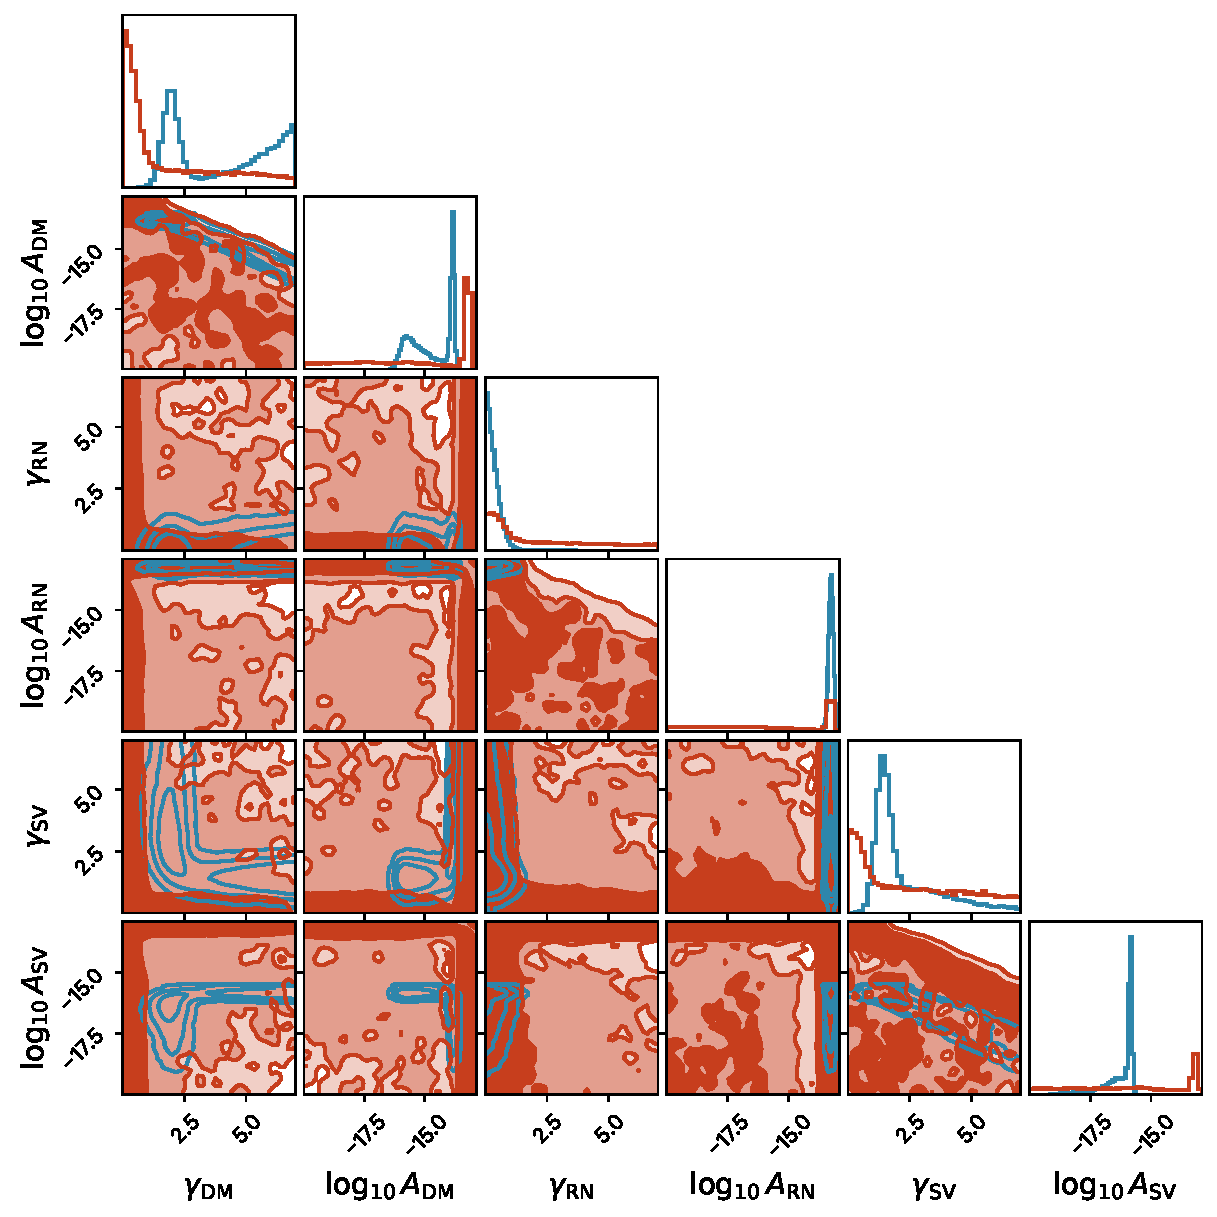
\includegraphics[height=0.8\textheight]{Figure/cap5/02_DR2low_vs_DR2newplus.pdf}
  \end{columns}
\end{frame}
